%%%%%%%%%%%%%%%%%%%%%%%%%%%%%%%%%%%%%%%%%%%%%%%%
% Tipo de documento y márgenes
%%%%%%%%%%%%%%%%%%%%%%%%%%%%%%%%%%%%%%%%%%%%%%%%
% Estilo de documento
\documentclass[letter,12pt]{article} 
% Márgenes
\usepackage[top = 2.5cm, bottom = 2.5cm, left = 2.5cm, right = 2.5cm]{geometry}  
%%%%%%%%%%%%%%%%%%%%%%%%%%%%%%%%%%%%%%%%%%%%%%%%
% Preparación de paquetes para el documento
%%%%%%%%%%%%%%%%%%%%%%%%%%%%%%%%%%%%%%%%%%%%%%%%
% Codificación
\usepackage[T1]{fontenc}
\usepackage[utf8]{inputenc}
% Se configura diccionario en español y en entorno de tablas aparecerá el nombre Tabla x
\usepackage[spanish,es-tabla]{babel}
% Se utilizará el punto decimal en lugar de coma para definir números con decimales
\spanishdecimal{.}
% Múltiples columnas
\usepackage{multirow} 
% Estilo de tablas
\usepackage{booktabs} 
% Incluir archivos PDF
\usepackage{graphicx} 
% PAra añadir figuras en formato EPS y transformarlas a PDF
\usepackage{epstopdf}
% Quita sangría al inicar párrado
\usepackage{setspace}
\setlength{\parindent}{0in}
% Obligar a figuras a insertarse donde el usuario indique
\usepackage{float}
% Para formato de encabezados
\usepackage{fancyhdr}
% Para símbolos y funciones matemáticas
\usepackage{amsmath,mathtools}
\usepackage{amsfonts}
\usepackage{amssymb}
% Para agregar colores predeterminados
\usepackage{xcolor}
% Para incluir algunas páginas de un archivo PDF
\usepackage{pdfpages}
\usepackage{soul}



%%%%%%%%%%%%%%%%%%%%%%%%%%%%%%%%%%%%%%%%%%%%%%%%
% Encabezado y pie de página
%%%%%%%%%%%%%%%%%%%%%%%%%%%%%%%%%%%%%%%%%%%%%%%%

\pagestyle{fancy} % Para personalizar encabezado

\fancyhf{} % Limpia encabezado y pie de página

\lhead{\footnotesize Proyecto  Bases de Datos } 			 % Coloca texto en la esquina superior izquierda, iniciales de la materia, semestre y grupo

\rhead{\footnotesize Luis Quintanar} % Coloca texto en la esquina superior derecha

\cfoot{\footnotesize \thepage} 	% Coloca número de página centrado en pie de página 

%%%%%%%%%%%%%%%%%%%%%%%%%%%%%%%%%%%%%%%%%%%%%%%%
% Contenido de documento
%%%%%%%%%%%%%%%%%%%%%%%%%%%%%%%%%%%%%%%%%%%%%%%%

\begin{document}

%%%%%%%%%%%%%%%%%%%%%%%%%%%%%%%%%%%%%%%%%%%%%%%%
% Título para la primera página
%%%%%%%%%%%%%%%%%%%%%%%%%%%%%%%%%%%%%%%%%%%%%%%%

\thispagestyle{empty} % Deshabilita el encabezado y pie de página para la primera página

\begin{tabular} {p{14cm} p{2cm}} 		% Inicia entorno de tabla para ordenar el contenido de datos de la materia
	&  \multirow{5}{*}{
\includegraphics[scale=0.11]{UNAM_INGENIERIA}}\\ % Se inserta el escudo de la facultad
{\large \bf Bases de Datos} & \\ 	% Nombre de la materia
{\large \bf Grupo: 01} & \\ 			% Número de grupo
UNAM / FI / DIE & \\				% División a la que pertenece la materia
Semestre 2021-2 &  \\					% Semestre actual
%&  \\ 
\hline 									% Se inserta línea horizonal
\end{tabular} 							% Finaliza entorno de tabla de datos de la materia

\vspace*{0.3cm} 						% Añade espacio entre datos de materia y nombre de tarea/práctica

\begin{center} 							% Inicia centrado de información
	{\Large \bf Proyecto} 	\\		% Se indica el número de tarea/práctica
	\vspace{2mm}
	
	{\bf Quintanar Ramirez Luis Enrique} % Nombre y apellido de integrantes del equipo
\end{center}  							% Finaliza centrado de información

%\vspace{0.3cm}							% Se deja espacio para comenzar a reportar resultados

%%%%%%%%%%%%%%%%%%%%%%%%%%%%%%%%%%%%%%%%%%%%%%%%
% A PARTIR DE AQUI SE REPORTAN SU TAREA/PRÁCTICA
%%%%%%%%%%%%%%%%%%%%%%%%%%%%%%%%%%%%%%%%%%%%%%%%
\section{Introducci\'on}
\subsection{Descripcion del an\'alisis del problema}
\subsubsection{Parte Uno}
Consiste en el diseño de una base de datos para una papeler\'ia.\\
Se desea tener almacenados datos como la {\bf raz\'on social, domicilio, nombre y
tel\'efonos} de los {\bf \ul{proveedores}, rfc, nombre, domicilio y al menos un email} de los
{\bf \ul{clientes}}. Es necesario tener un {\bf \ul{inventario}} de los {\bf \ul{productos}} 
que se venden, en el
que debe guardarse el {\bf código de barras, precio al que fue comprado el producto,
fecha de compra y cantidad de ejemplares en la bodega (stock)}. Se desea guardar
la {\bf marca, descripci\'on y precio} de los {\bf \ul{regalos}, \ul{art\'iculos de papeleria}, 
\ul{impresiones} y
\ul{recargas}}, siempre y cuando se tenga su correspondiente registro en el inventario.
Debe tambi\'en guardarse el {\bf número de venta, fecha de venta y la cantidad total
a pagar de la \ul{venta}, as\'i como la cantidad de cada art\'iculo y precio total a pagar
por art\'iculo}. Adem\'as, se requiere que:
\begin{itemize}
\item Al recibir un codigo de barras, regrese su utilidad.
\item Cada que haya una venta decrementar su stock (Si llega a cero, abortar. Si hay menos de tres, emitir mensaje).
\item Dada una fecha o una fecha de inicion y de fin, regresar la cantidad total que se vendio en esa fecha/periodo.
\item De manera automatica se genere una vista que se asemeje a una factura.
\item Crear al menos un índice. Justificar la elecci\'on.
\end{itemize}
\subsubsection{Parte Dos}
Una vez diseñada y lista la base de datos, se deber\'a crear una interfaz gráfica vía app movil o web, que permita:
\begin{enumerate}
\item Agregar informacion de un cliente.
\item Ingresar una venta de hasta tres articulos e ingresar la informacion en la base de datos.
\end{enumerate}
\newpage
\subsection{Objetivos}
\begin{itemize}
\item Analizar y describir el funcionamiento para la creación de la BD
\item Crear una BD funcional y que aplique correctamente al problema 
\item Crear una aplicación para la parte dos
\end{itemize}
\subsection{Propuesta de soluci\'on}
Cada una de las propuestas serán detalladas en la sección de diseño
\begin{itemize}
\item Para el analisis y descripcion del funcionamiento del sistema deseado, se realizará el modelos entidad relacion y el modelo relacional.
\item Una vez realizados los modelos ME y MER, crearemos la base de datos, siguiendo la descipción de los mismos
\item Para la parte dos, elegí la creación de un sistema realizado en lenguaje C, debido a que cuenta con una extension que permite manejar postgresql y además de que me encuentro demasiado familiarizado al lenguaje
\end{itemize}

\section{Plan de Trabajo}
Para elaborar de la mejor manera el sistema deseado, el trabajo se realizará en las siguientes fases de trabajo:
\begin{itemize}
\item Análisis de requerimientos. Recopilación de los requisitos, especificaciones y restricciones
\item Diseño Conceptual. Descripción concisa de los requisitos mediante el MER
\item Diseño Lógico. Transformación del MER en un modelo físico (MR)
\item Diseño Físico. Adaptación del modelo físico al gestor de bases de datos
\item Implementación y optimización. Procesamiento de la consulta. Procesamientos de vistas. Administración de Seguridad.Creación del sistema en C
\end{itemize}

\newpage
\section{Diseño}
\subsection{Análisis de requerimientos}
Basandome en el documento llamado ProyectoFinalBD.pdf escrito por el Ing. Fernando Arreola en Junio de 2021, para la parte uno, observamos que existen varias entidades, con sus atributos, relacionadas entre sí. En primer lugar, encontramos a los proveedores, que cuentan con razón social, domicilio, nombre y telefonos. Encontramos, además, a los clientes, de los cuales se requiere el RFC, nombre, domicilio, y al menos un email. \\
Otra entidad que vemos es la de producto, que tiene un codigo de barras, precio, marca y descripcion, ademas de una categoria que puede ser articulo de papeleria o regalo. Dentro del inventario, guardaremos el codigo de barras del producto, la fecha de compra, el precio de compra y el stock.\\
Además, se presentan los servicios, que aunque no se describan como tal, esos no los encontramos en el inventario, por lo que me pareció que sería mejor separarlo y en ellos están las recargas y las impresiones, ambas cuentan con descripción y precio, aunque recargas cuenta con compañia e impresiones con el tipo de impresion(b/n o a color) y tamaño de hoja (A0,A1,...). Y se requiere guardar el numero de venta, la fecha de venta, la cantidad total, la cantidad de cada articulo y el precio total por articulo. Todo esto será de utilidad en el diseño conceptual y el diseño logico más adelante.\\
En especificaciones y restricciones tenemos que:
\begin{itemize}
\item Al recibir un codigo de barras, regresar la utilidad
\item Cada que haya una venta, decrementar el stock
\item Dada una fecha o rango de fecha, regresar las ventas
\item Permitir obtener el nombre de aquellos productos con menos de 3 en stock
\item Crear al menos un indice
\item Generar vista de manera automática parecida a una factura
\item Los requerimientos deben ser realizados por medio de PgSQL
\item El formato de venta debe ser "VENT- 001"
\item El atributo domicilio esta conformado por estado, CP, colonia, calle y numero
\end{itemize}
\subsection{Diseño Conceptual}
Teniendo ya el análisis de requerimientos, comencé a unir la información en el MER, cada entidad con sus respectivos atributos. Obteniendo los siguiente:
\begin{center}
\begin{figure}[H]
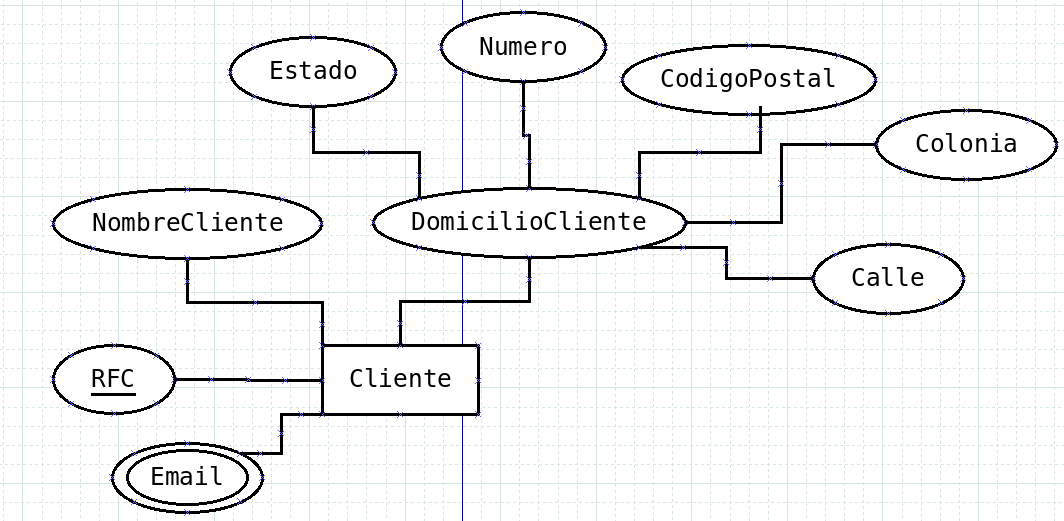
\includegraphics[scale=.4]{cliente.png}
\caption{Entidad cliente}
\end{figure}
\begin{figure}[H]
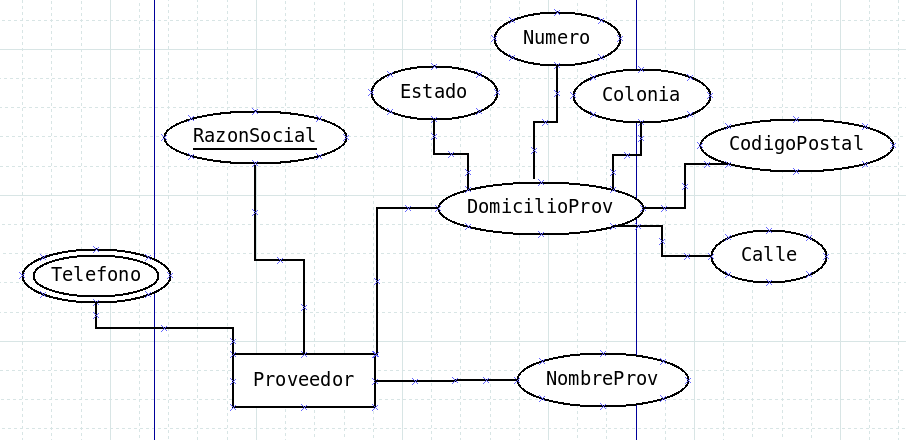
\includegraphics[scale=.45]{proveedor.png}
\caption{Entidad proveedor}
\end{figure}
\newpage
\begin{figure}[H]
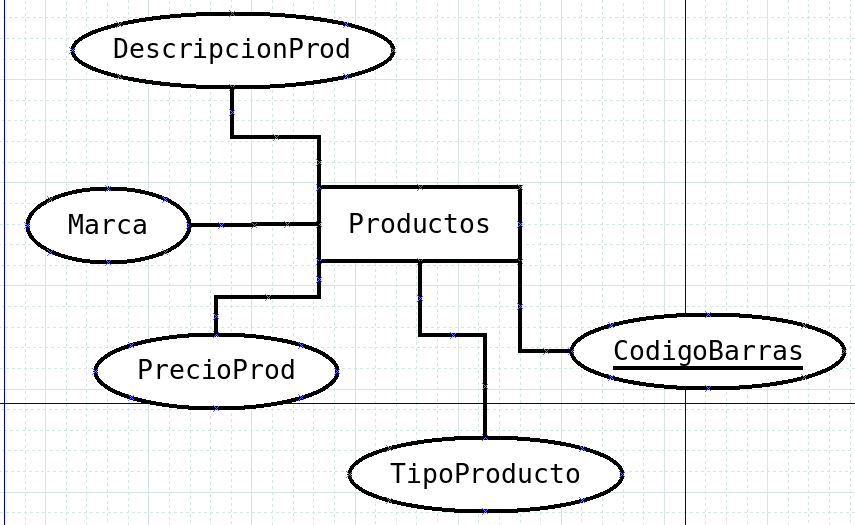
\includegraphics[scale=.45]{productos.png}
\caption{Entidad productos}
\end{figure}
\begin{figure}[H]
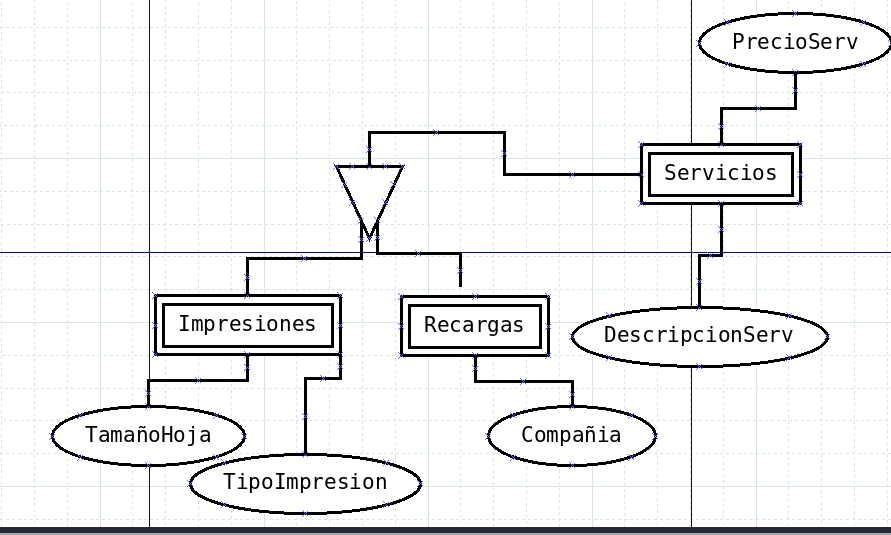
\includegraphics[scale=.45]{servicios.png}
\caption{Entidad servicios}
\end{figure}
\newpage
\begin{figure}[H]
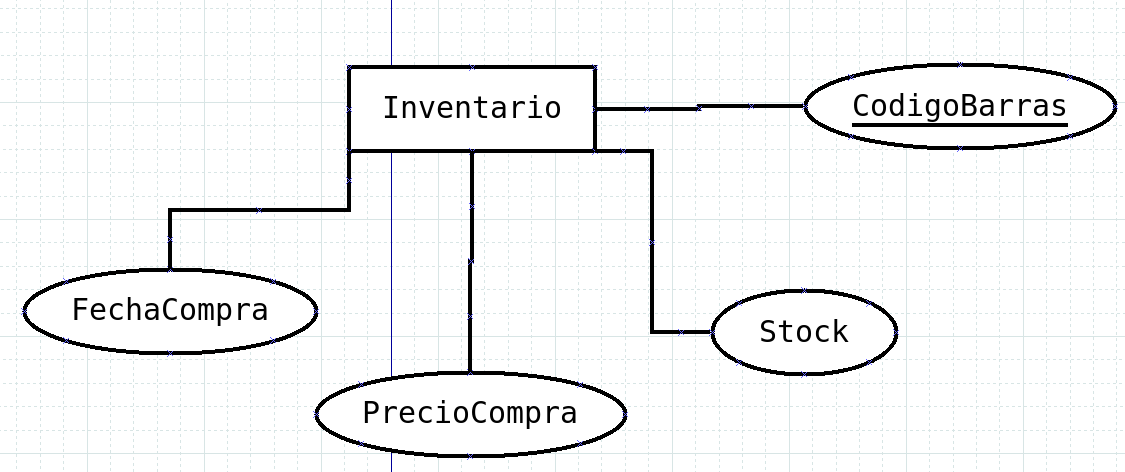
\includegraphics[scale=.4]{inventario.png}
\caption{Entidad inventario}
\end{figure}
\begin{figure}[H]
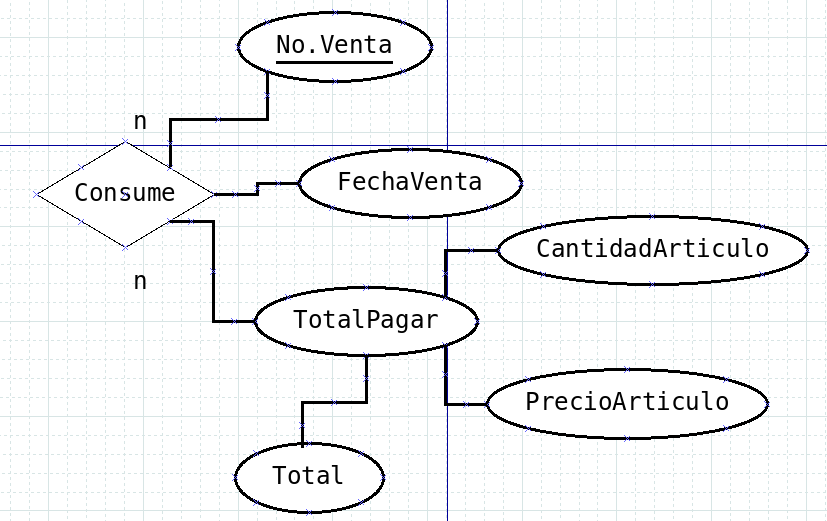
\includegraphics[scale=.45]{venta.png}
\caption{Relacion consumo}
\end{figure}
\newpage
\end{center}
Como podemos observar, consumo no es una entidad, si no una relación con atributos. Que a mí parecer fue la mejor solución a este problema. Además vemos que cada entidad se relaciona con otras quedando de la siguiente manera:\\ \\
Cliente (consume) => Producto y/o Servicios\\
Productos (existe en) => Inventario\\
Proveedor (surte) => Inventario\\
\begin{center}
\begin{figure}[H]
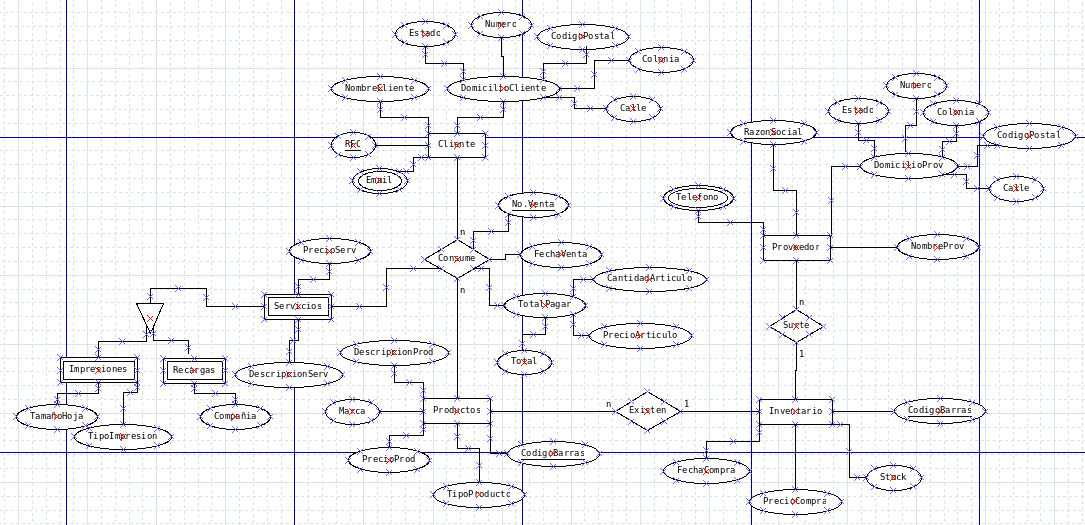
\includegraphics[scale=.45]{MER.png}
\caption{MER completo}
\end{figure}
\end{center}
\newpage
\subsection{Diseño Logico}
Teniendo el MER, lo adaptamos al un diseño logico, más orientado a la creación de la Base de Datos. Quedando de la siguiente manera:
\begin{center}
\begin{figure}[H]
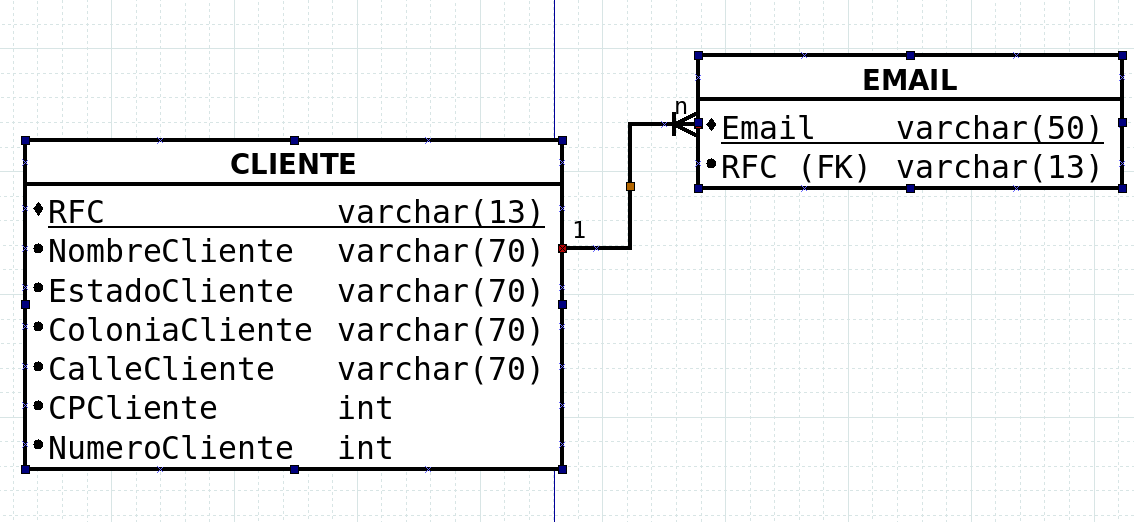
\includegraphics[scale=.45]{clienteMR.png}
\caption{Cliente MR}
\end{figure}
\begin{figure}[H]
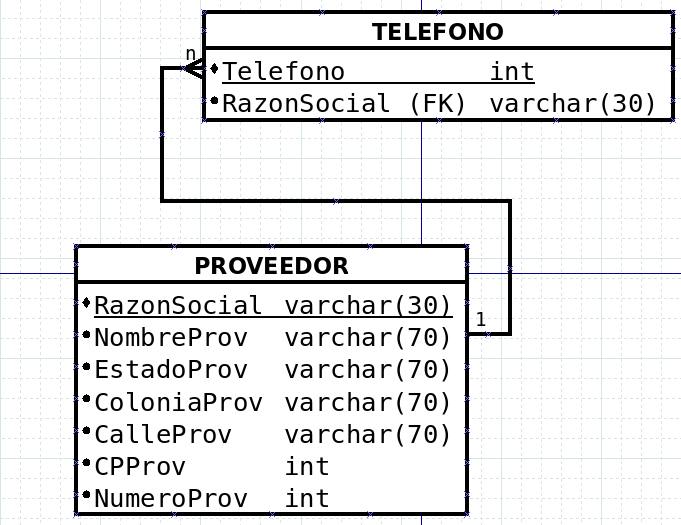
\includegraphics[scale=.45]{proveedorMR.png}
\caption{Proveedor MR}
\end{figure}
\newpage
\begin{figure}[H]
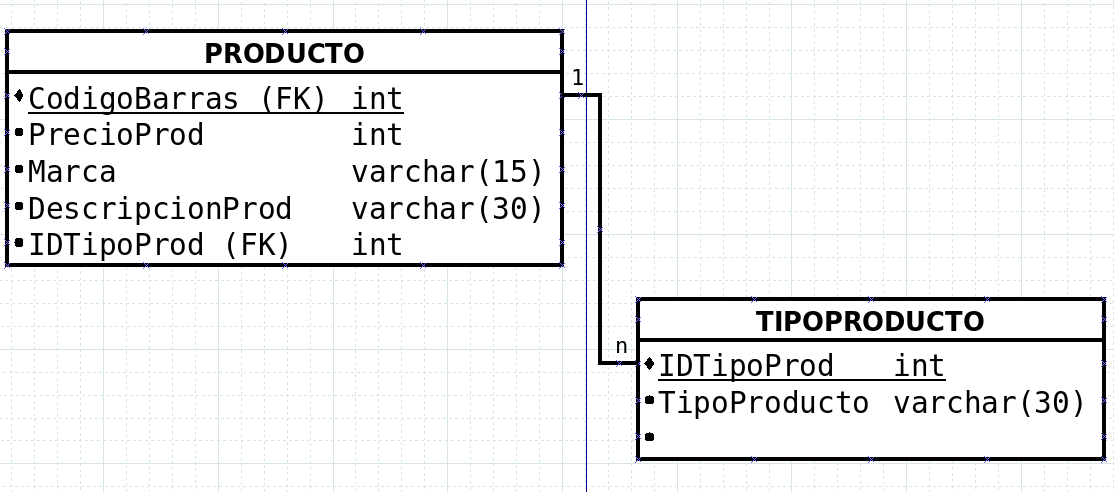
\includegraphics[scale=.45]{productoMR.png}
\caption{Producto MR}
\end{figure}
\begin{figure}[H]
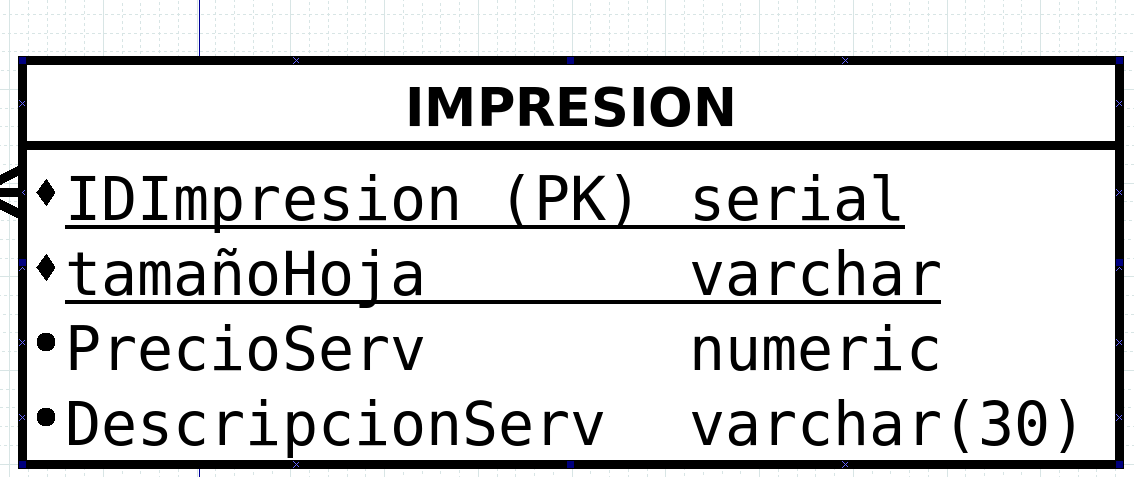
\includegraphics[scale=.45]{impresionMR.png}
\caption{Impresion MR}
\end{figure}
\newpage
\begin{figure}[H]
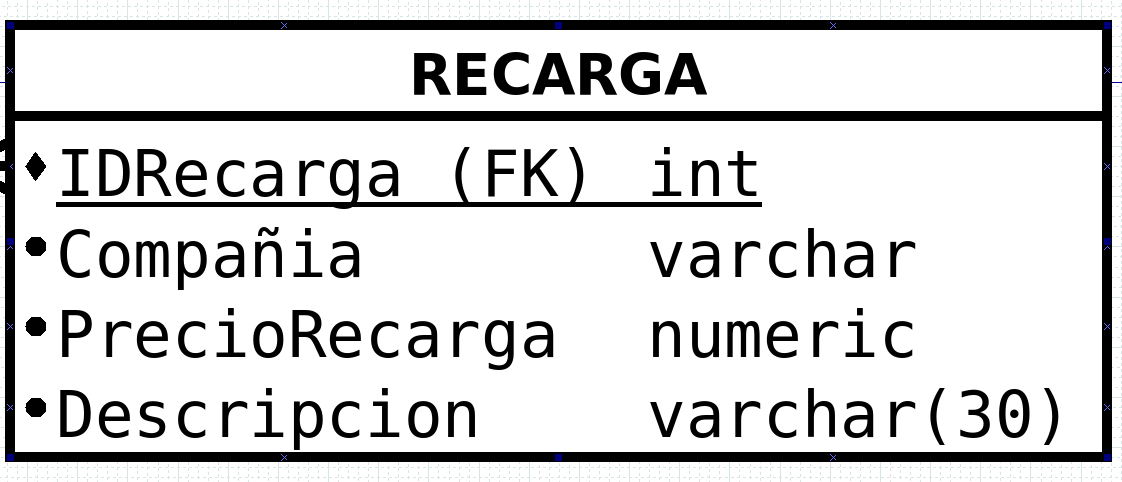
\includegraphics[scale=.45]{recargaMR.png}
\caption{Recarga MR}
\end{figure}
\begin{figure}[H]
\includegraphics[scale=.45]{inventarioMR.png}
\caption{Inventario MR}
\end{figure}
\newpage
\begin{figure}[H]
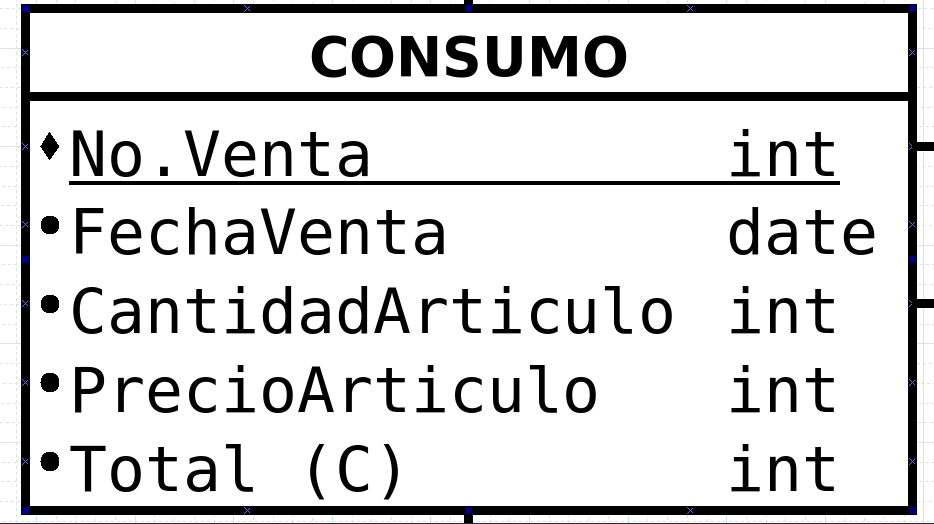
\includegraphics[scale=.45]{ventaMR.png}
\caption{Consumo MR}
\end{figure}
\begin{figure}[H]
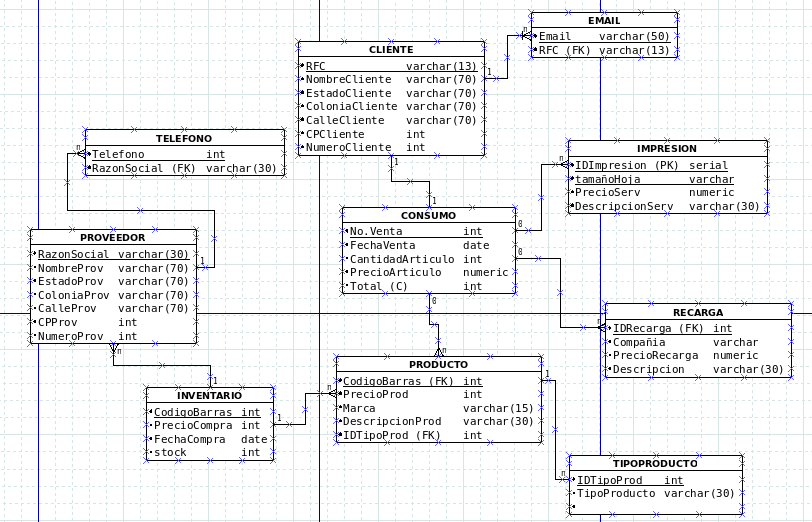
\includegraphics[scale=.45]{MR.png}
\caption{MR completo}
\end{figure}
\end{center}
Observamos que tanto en email como en telefono son dos tablas aparte de cliente y proveedor, debido a que son atributos multivaluados y pueden contener mas de un telefono o email, por lo tanto, hay que normalizar la tabla
\newpage
\subsection{Diseño Físico}
Una vez que tenemos el Diseño Lógico, adaptamos las tablas que observamos al manejador PostgreSQL, podemos observar el resultado en el archivo ScriptDB.sql
\begin{center}
\begin{figure}[H]
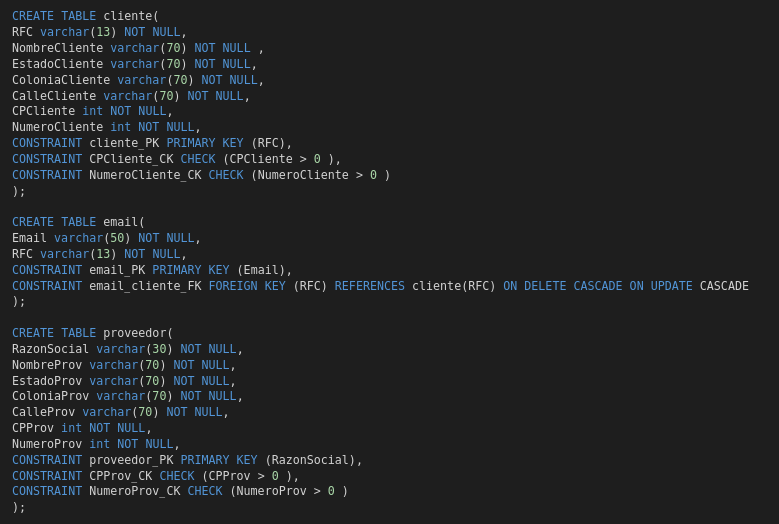
\includegraphics[scale=.5]{clienteEmailProveedorBD.png}
\caption{Cliente, Email, Proveedor en PgSQL}
\end{figure}
\begin{figure}[H]
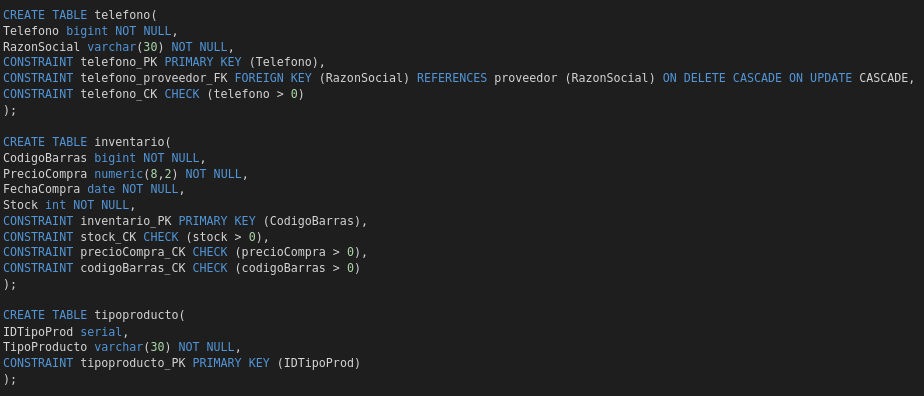
\includegraphics[scale=.45]{telefonoInventarioBD.png}
\caption{Telefono, Inventario, TipoProducto en PgSQL}
\end{figure}
\begin{figure}[H]
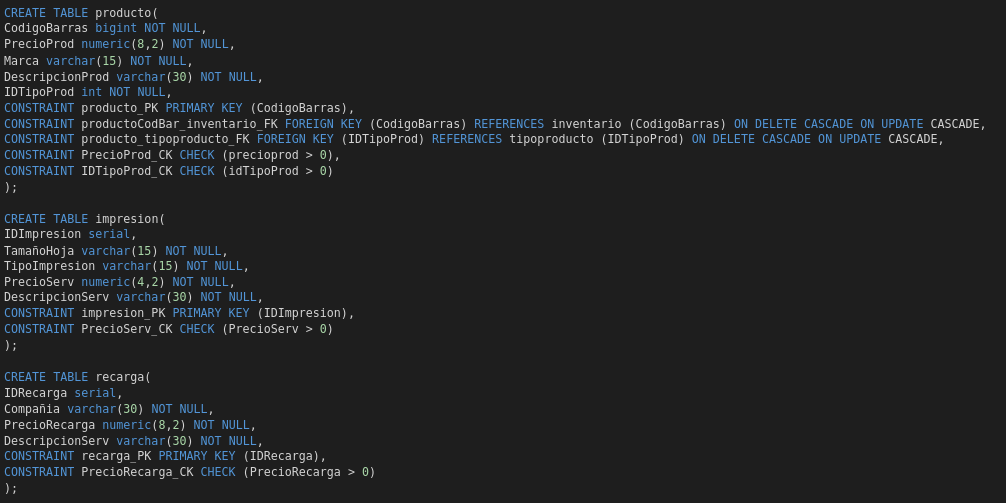
\includegraphics[scale=.45]{productoImpresionRecargaBD.png}
\caption{Producto, Impresion, Recarga en PgSQL}
\end{figure}
\begin{figure}[H]
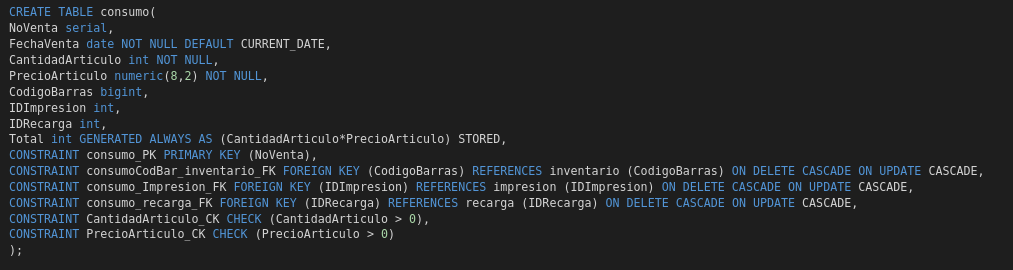
\includegraphics[scale=.45]{consumoBD.png}
\caption{Consumo en PgSQL}
\end{figure}
\end{center}
\subsection{Implementacion y optimización}
Contando ya con la base de datos hecha con sus respectivas tablas y los datos de ScriptInfo.sql cargados. En cuestiones de seguridad, agregamos anteriormente todas las restricciones de llaves primarias, llaves foranea, y algunos checks para que los datos ingresados sean correctos, por ejemplo, en los precios, verificamos que sean solo numeros positivos, asi como en el codigo de barras. \\
Agregamos vistas que nos permiten tener mejor control sobre lo que se muestra al usuario. Además de que agregamos el index, en el codigo de barras en la tabla inventario, debido a que estamos constantemente accediendo a esa información, para realizar ventas, mostrar inventario, mostrar productos, etc. Además de que con el comando EXPLAIN pude observar que se veía una mejora en el tiempo de consulta, a diferencia de si se agregaba en otros datos como RFC en cliente o Razon Social en proveedor. Claro, tambien se cuentan con los indices de cada una de las llaves primarias de tipo UNIQUE. \\
Agregué una funcion y un trigger que nos permite decrementar el inventario al realizar una compra. Mejor explicado en la seccion de implementación.\\
Contando ya con todo lo relacionado a la base de datos, me dí a la tarea de realizar un sistema en C, para tener mejor control de los datos, y una interfaz que limite al usuario y hacer más "seguro" el sistema. El cual explicaré de manera más detallada en la sección de Presentacion.
\section{Implementaci\'on}
Como se mencionó anteriormente, generamos varias vistas que mostrarán al usuario de mejor manera lo que desea, al querer realizar una compra, mostrará los productos, las recargas o las impresiones, además generamos otra vista para el inventario que agrega la utilidad para tener mejor visión, y otras dos para ver la informaciín de los clientes y los proveedores y la más importante, la vista que genere una salida similar a la de una factura. \\
También incluí una función para decrementar el stock del inventario al realizar una compra, como se requería según el documento y su trigger para realizarlo después de realizar una venta
\begin{center}
\begin{figure}[H]
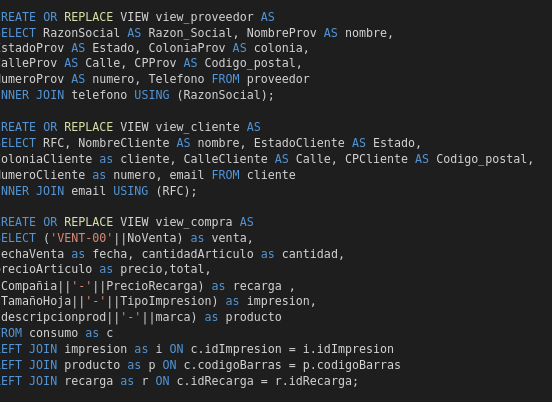
\includegraphics[scale=.8]{viewProveedorClienteCompra.png}
\caption{Codigo Views Proveedor, Cliente, Compra}
\end{figure}

\begin{figure}[H]
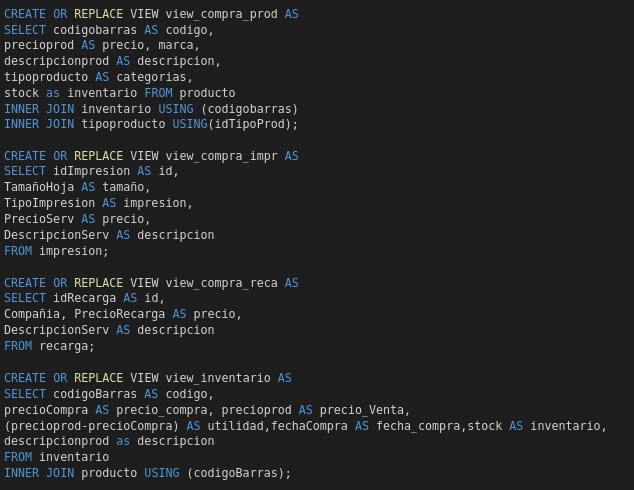
\includegraphics[scale=.8]{viewProdRecargaImpresionInventario.png}
\caption{Codigo Views Compra de Recarga, Impresion, Producto e Inventario}
\end{figure}
\newpage
\begin{figure}[H]
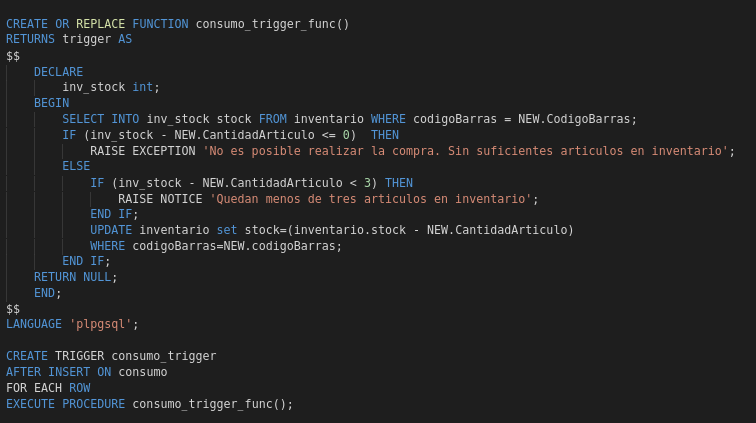
\includegraphics[scale=.7]{function_Trigger.png}
\caption{Codigo Funcion de decremento del Stock y su trigger}
\end{figure}
\end{center}
Cuyos resultados pueden verse como:
\begin{figure}[H]
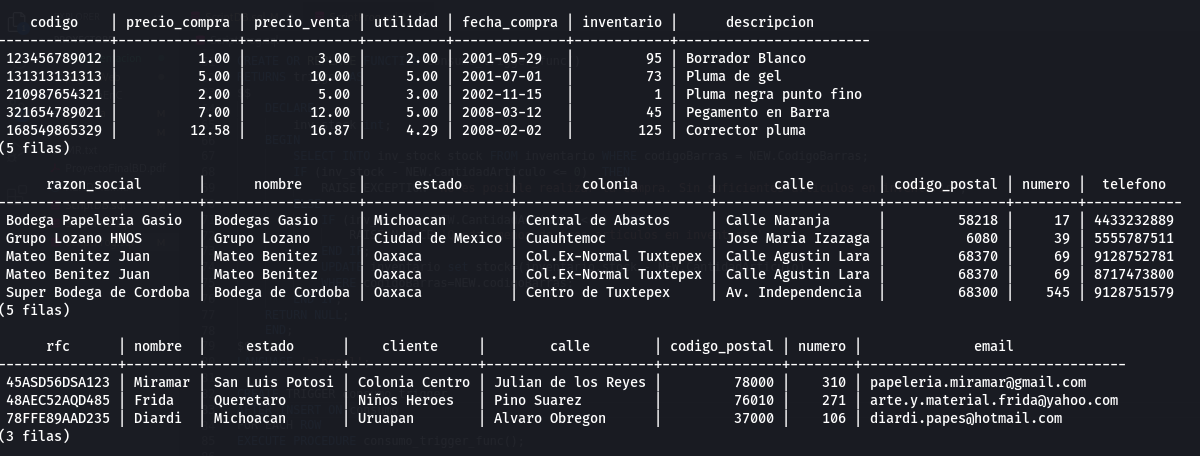
\includegraphics[scale=.44]{viewInvenProvClienteR.png}
\caption{Resultado views Inventario, Proveedores, Clientes}
\end{figure}
\newpage
\begin{figure}[H]
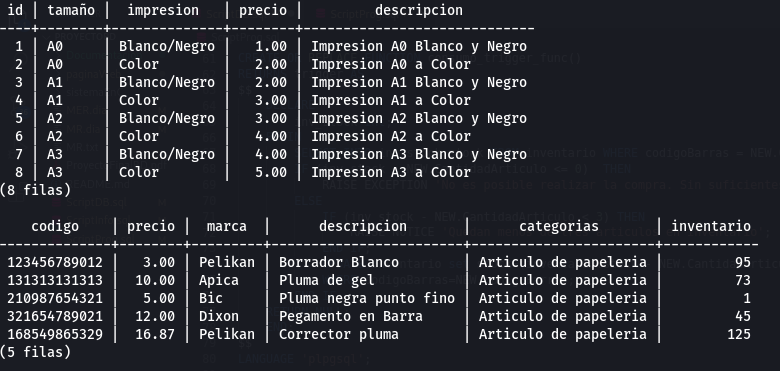
\includegraphics[scale=.60]{viewImpreProdR.png}
\caption{Resultado views Impresiones Productos}
\end{figure}
\begin{figure}[H]
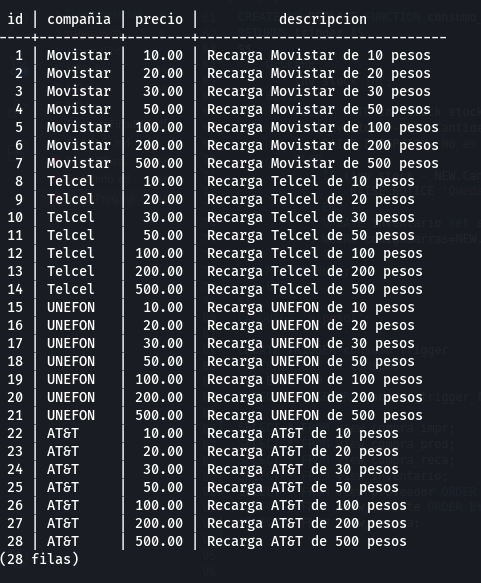
\includegraphics[scale=.6]{viewRecargaR.png}
\caption{Resultado views Recargas}
\end{figure}
\begin{figure}[H]
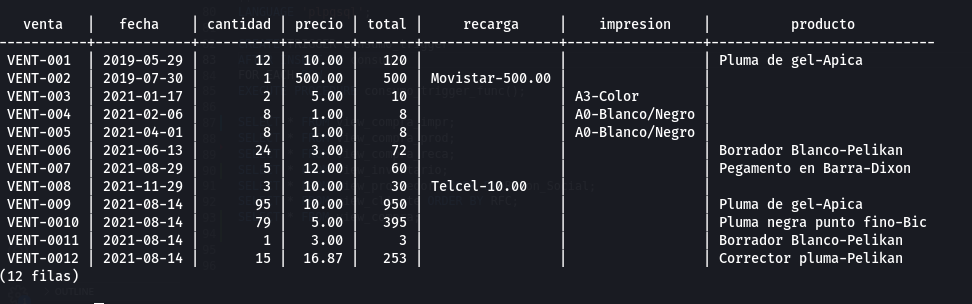
\includegraphics[scale=.5]{viewConsumoR.png}
\caption{Resultado views Compras}
\end{figure}
\section{Presentaci\'on}
Se realizó un sistema en lenguaje C, que a grandes rasgos, nos conecta a la base de datos, despliega un menu que nos permite realizar varias acciones:
\begin{itemize}
\item Registar Cliente.\\
Al ingresar en esta opción, nos pide los datos del cliente: RFC, Nombre, Estado, Colonia, Calle, CP, Numero e email. E ingresa los datos en la base de datos en cliente e email
\item Registrar Proveedor\\
Solicita los datos del proveedor: Razon Social, Nombre, Estado, Colonia, Calle, CP Numero y telefonos e ingresa los datos en las tablas proveedor y telefonos
\item Registrar Producto\\
Pide el ingreso de la información del producto: Codigo de Barras, Precio de compra, Fecha de compra, Stock, Precio de Venta, Marca y descripción del producto
\item Realizar Compra\\
Muesta tres opciones más:
\begin{itemize}
\item Comprar articulos de papeleria/regalos\\
Muestra los articulos con más de un producto en inventario. Debido a que no se puede dejar en cero algun artículo debido a las restricciones del usuario, pide el codigo de barras y la cantidad de articulos deseados.
\item Realizar Recargas\\
Muestra las posibles recargas y pide una al usuario. Ingresa los datos en ventas
\item Impresiones\\
Muestra las posibles Impresiones y pide una al usuario. Ingresa los datos en ventas
\end{itemize}
\item Mostrar Inventario\\
Despliega la infomacion de inventario de la base de datos, usando los views creados
\newpage
\item Mostrar Compras\\
Despliega un submenu que  muestra todas las ventas, las ventas de una fecha dada o las ventas en un intervalo de fechas
\item Mostrar Clientes\\
Despliega una lista de la informacion de los clientes.
\item Mostrar Provedores\\
Muestra una lista con la informacion de los proveedores.
\item Salir\\
Cierra la conexión a la base de datos y finaliza el programa
\end{itemize}
Observando su comportamiento
\begin{center}
\begin{figure}[H]
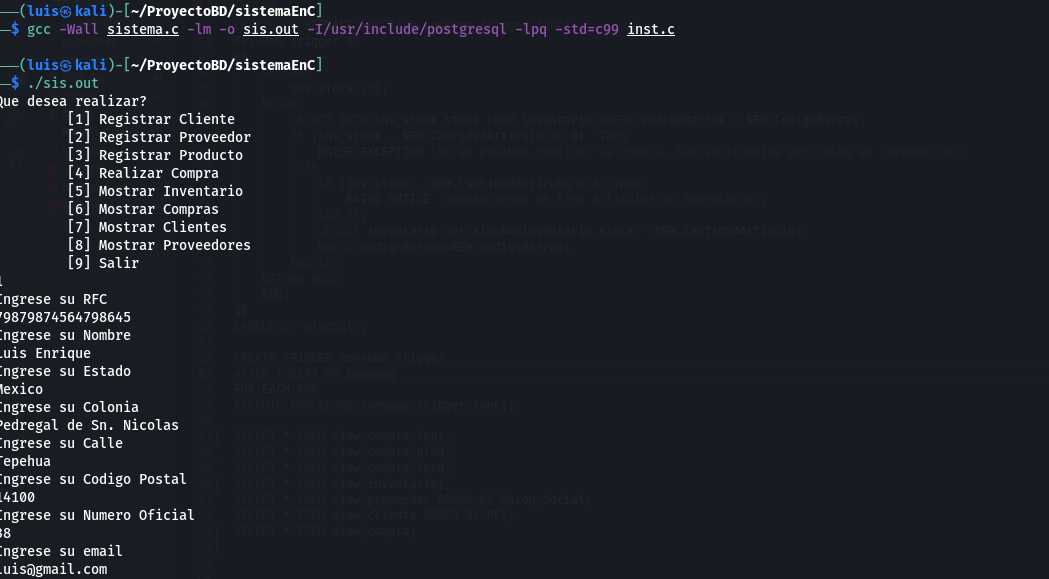
\includegraphics[scale=.44]{func1.png}
\caption{Registro Cliente}
\end{figure}
\begin{figure}[H]
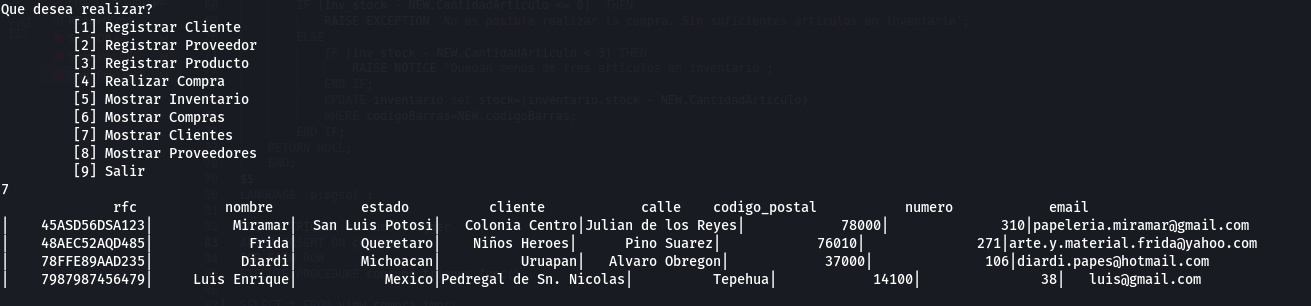
\includegraphics[scale=.35]{func1-1.png}
\caption{Muestra los clientes, observamos al cliente ingresado anteriormente}
\end{figure}
\begin{figure}[H]
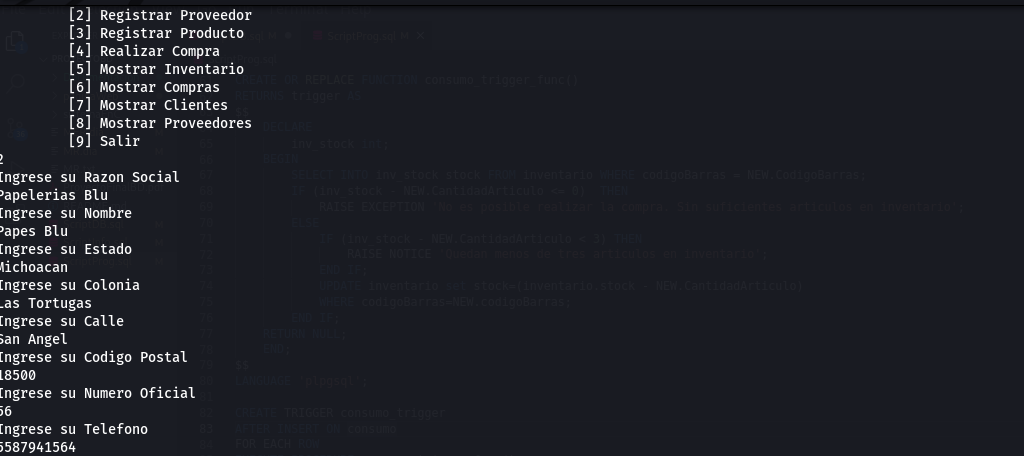
\includegraphics[scale=.45]{func2.png}
\caption{Registro Proveedor}
\end{figure}
\begin{figure}[H]
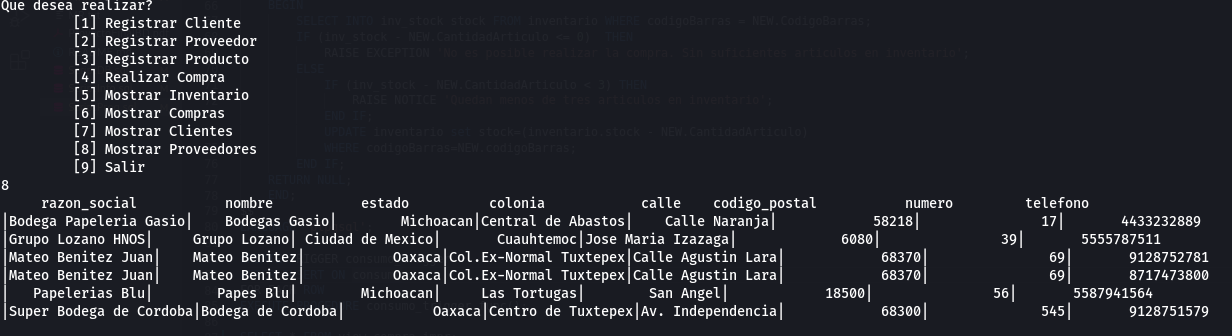
\includegraphics[scale=.40]{func2-1.png}
\caption{Muestra los proveedores, observamos al proveedor ingresado anteriormente}
\end{figure}
\begin{figure}[H]
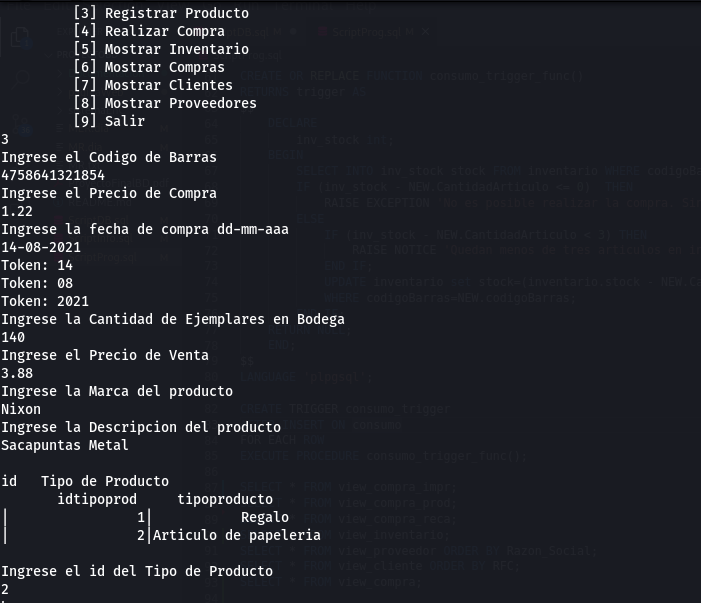
\includegraphics[scale=.6]{func3.png}
\caption{Registro Producto}
\end{figure}
\begin{figure}[H]
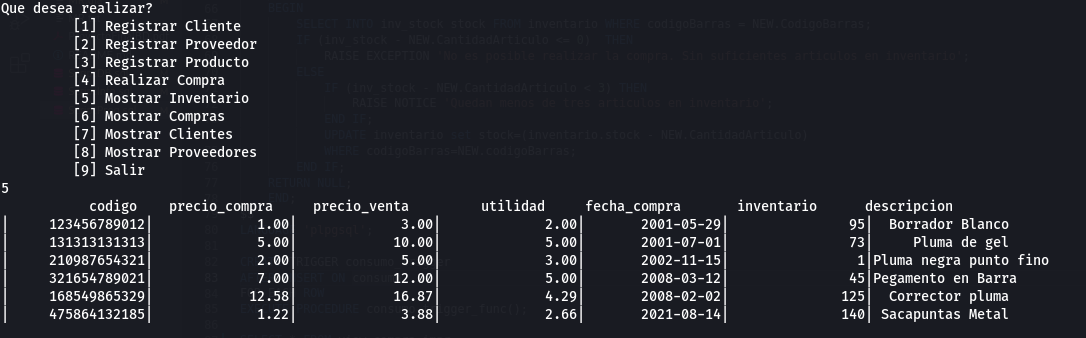
\includegraphics[scale=.40]{func3-1.png}
\caption{Muestra el inventario, observamos el producto ingresado anteriormente}
\end{figure}
\begin{figure}[H]
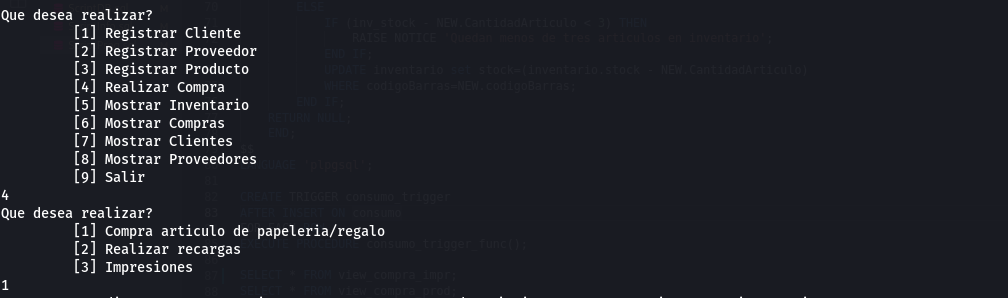
\includegraphics[scale=.45]{func4-1.png}
\caption{Compra Producto 1}
\end{figure}
\begin{figure}[H]
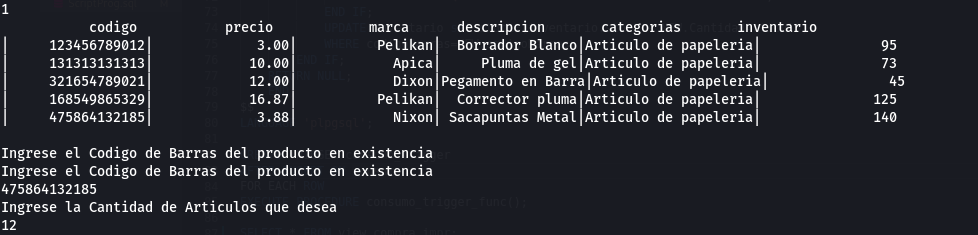
\includegraphics[scale=.45]{func4-2.png}
\caption{Compra Producto 2}
\end{figure}
\begin{figure}[H]
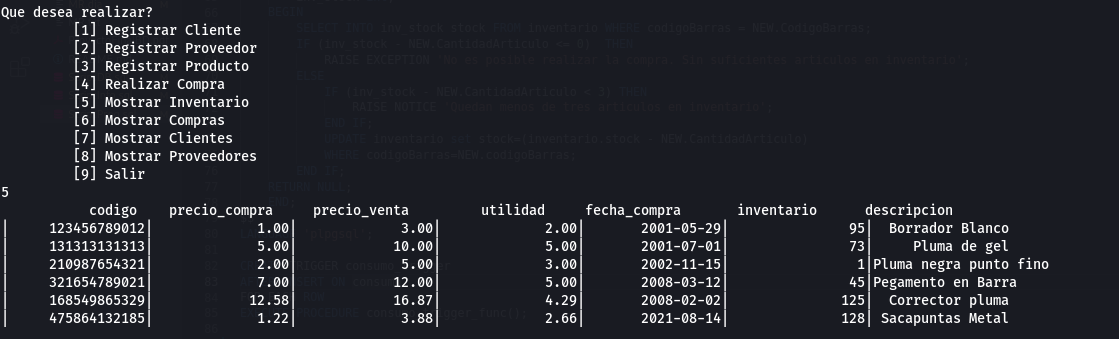
\includegraphics[scale=.40]{func4-3.png}
\caption{Muestra inventario. Stock en producto comprado reducido}
\end{figure}
\end{center}
\newpage
\section{Conclusiones}
Una de las partes que tuve más dificultades, fue en la parte de Diseño, tanto conceptual como lógico debido a que la adaptacion de los requerimientos y abstraccion del sistema se me complicó. Especialmente en la parte de recargas e impresiones, pues no sabía dónde acomodarlos, hasta que identifiqué que no eran productos más bien, servicios. De ahí en adelante, la parte de diseño físico y adaptacion a PgSQL, se me hizo más fácil. Y creo que fue una buena elección de mi parte, continuar programando en C y desarrolarlo en sistemas Linux, debido a que ya tengo un gran recorrido en ese lenguaje, y se adaptó perfectamente a la base de datos, además de que en Linux algunas instalaciones y configuraciones fueron más sencillas de resolver. Sin embargo, tuve algunos problemas al principio para conectarme a la BD, debido a las contraseñas con el usuario postgres, así que creé otro usuario especial para la base y le di sus debidas configuraciones para ingresar a los servidores. Al trabajar sólo, la ventaja fue el tiempo, debido a que no perdía tanto tiempo en reuniones o en intercambio de opiniones, y justo por eso, tuve una desventaja al observar las otras posibles opciones para solucionar el problema. Sin embargo, a mi consideracion creo que los puntos se cumplieron adecuadamente.

\end{document}